\documentclass[12pt, a4paper]{article}
\usepackage[english, russian]{babel}
\usepackage[T2A]{fontenc}
\usepackage[utf8]{inputenc}
\usepackage[left=2cm,right=2cm,top=2cm,bottom=2cm,bindingoffset=0mm]{geometry}
\usepackage{titlesec}
\usepackage{amsmath}
\usepackage{setspace}
\usepackage[pdftex]{graphicx}
\usepackage{dsfont}
\usepackage{comment}
\usepackage[unicode, pdftex]{hyperref}
\usepackage{fancyhdr}
\usepackage{colortbl}

\graphicspath{{C:/Users/user/Desktop/NLP_foto}}
\newtheorem{theorem}{$\quad$ Теорема}
\setlength{\parindent}{5mm}
\linespread{1.4}


\begin{document}

\pagestyle{fancy}
\fancyhf{}
\renewcommand{\headrulewidth}{0pt}

\begin{center}
САНКТ-ПЕТЕРБУРГСКИЙ ГОСУДАРСТВЕННЫЙ УНИВЕРСИТЕТ\\
Направление: 01.03.02 Прикладная математика и информатика \\
Кафедра технологии программирования \\

\vspace*{2cm}
\large \textbf{ОТЧЕТ О НАУЧНО-ИССЛЕДОВАТЕЛЬСКОЙ РАБОТЕ}
\end{center}
\vspace*{2cm}

\hspace*{0.5cm}
Tема задания: Исследование алгоритмов лемматизации
\vspace*{1cm}

\hspace*{0.5cm}
Выполнил: Смирнов Алексей Артёмович, группа 21.Б02-пу 
\vspace*{1cm}

\hspace*{0.5cm}
Руководитель научно- \\
\hspace*{1cm} исследовательской работы: Блеканов Иван Станиславович, кандидат технических \\\hspace*{1cm} наук, доцент, заведующий кафедрой технологии программирования
 
 
\vspace*{10cm}
\begin{center}
САНКТ-ПЕТЕРБУРГ \\
2023
\end{center}

\newpage

\renewcommand{\contentsname}{\begin{center}Содержание\end{center}}
\tableofcontents

\newpage

\fancyfoot[C]{\thepage}

\section{Введение}
\quad Данная работа посвящена изучению технологии Natural Language Processing(NLP) - одной из важнейших отраслей машинного обучения, дающую возможность обработки и создания информации на естественном языке. Мы рассмотрим лишь часть NLP, называемую лемматизацией, получим численную оценку нескольких популярных алгоритмов на реальных данных, что позволит оценить данную задачу со всех сторон.

Лемматизация - процесс приведения словоформы к лемме, то есть к её нормальной форме. В русском языке при построении текста используются различные формы слова в зависимости от контекста, но в большинстве случаев идею текста можно понять заменив все слова на их нормальные формы, тем самым можно облегчить задачу компьютеру, уменьшив количество вариаций входных данных. Например все формы: \text{'ездил', 'ездила', 'ездили'} после лемматизации становятся равными \text{'ездить'}. Конечно, хоть лемматизация упрощает работу с текстом, после ее выполнения мы теряем часть информации заложенной изначально, но для некоторых задач, например таких как классификация и кластеризация документов, необязательно знать всю информацию заложенную в нем, достаточно различать лишь те признаки, которые позволяют определять объекты одного класса.

\subsection{Актуальность работы}
\quad Исследование различных алгоритмов лемматизации может помочь наиболее эффективно подбирать соответвующие методы в зависимости от конкретных задач на основе знания их преймуществ и недостатков, а также понимать наиболее важные проблемы и их решения в данной области. Технология NLP широко применяется в браузерах, например, при обработке запроса пользователя, извлекая ключевые идеи текста запроса, а также при индексировании вебстраниц, исправляя ошибки написания документов. Усовершенствование технологии NLP может привести к переходу к Natural Language Understanding(NLU), сделав возможным обработку не самого языка, а образов, которые закладывает человек при написании текста. 
Также ныне реализованные языковые модели, способные общаться с человеком, поддерживая разговоры на определенную тему, показывают практическую применимость рассматриваемых методов в области машинного обучания.

\subsection{Цель и задачи работы}
\quad Цель данной работы в описании и практической оценке популярных алгоритмов лемматизации для русского языка, сравнении их преймуществ и недостатков, а также в рассмотрении возможностей их усовершенствования с примерами фреймворков, использующихся на практике.

\section{Различные метрики символьных последовательностей}
\quad Основная идея ввода различных метрических хактеристик состоит в том, что мы хотим представить слово как элемент некоторого метрического пространства. Если мы будем знать все нормальные формы всех слов, то есть иметь словарь языка, то, в предположении, что словоформа не сильно отличается от своей нормальной формы по введеной метрике, мы сможем найти ближайший элемент из словаря, который и будет являться леммой.

Стоит отметить, что в современных алгоритмах данные метрики используются лишь как один из этапов приведения слова к лемме. Рассмотрим несколько примеров таких метрик.

\subsection{Расстояние Левенштейна}
\quad Расстояние Левенштейна - метрика, определяющая расстояние между символьными последовательностями по минимальному количеству односимвольных операций: \textbf{вставок}, \textbf{удалений} и \textbf{замены}, необходимых для приведения одной последовательности к другой. 

Для определения минимального количества операций определенных выше, необходимо вычислить значение $D(m, n)$, где $m$ - длина слова $\:W_1$, $n$ - длина слова $\:W_2$. Значение $\;D(m, n)\;$ можно вычислить по следующей реккурентной формуле:

$$
\label{2.1}
D(i, j) = 
\begin{cases} 
\max(i, j), \quad \quad \quad \quad \quad \; \; \min(i, j) = 0  \\
\min( \quad \quad \quad  \quad  \quad \quad \quad \quad \text{иначе}\\
\quad D(i, j - 1) + 1, \\
\quad D(i - 1, j) + 1, \\
\quad D(i - 1, j - 1) + (W_1[i] \: \neq \: W_2[j]) \\
\quad )
\end{cases}
\eqno(2.1)
$$

$$
(W_1[i] \: \neq \: W_2 [j]) = 
\begin{cases} 
1, \quad \text{если i-тый символ} \;\; W_1 \;\; \text{неравен j-тому символу}\;\; W_2 \\
0  \quad \; \text{иначе}
\end{cases}
$$

Из вида формулы $(\ref{2.1})$ можно получить оценку сложности по времени и памяти для  алгоритма, который принимал бы на вход слово длины $n$ и по известному словарю лемм языка, с количеством слов -  $N$, выдавал ближайшую лемму по расстоянию Левенштейна, которую и будем считать нормальной формой данного слова. Значение оценки по времени есть $O(Nna)$, где $a$ - средняя длина слова в словаре, по памяти - $O(na)$, которую можно сократить до $O(\min\{n, a\})$, так как нас не интересует способ приведения строк к равенству.

Сразу можно увидеть серьезный идейный недостаток данной метрики для задачи лемматизации, а именно то, что расстояние между короткими несовпадающими словами может быть довольно мало, из-за чего результат лемматизации отдельных коротких слов может быть сильно ошибочным, искажающим суть текста.

\subsection{Расстояние Джаро}
\quad Расстояние Джаро - метрика, определяющая расстояние между символьными последовательностями по их схожести. В отличии от расстояния Левенштейна, чем больше значение метрики, тем более строки похожи друг на друга, так как метрика основана на совпадающих символах.

Расстояние Джаро $\:d_j\:$ между двумя словами $\:W_1\;$ и $\:W_2\;$ определяется по следующей формуле:

$$
\label{2.2}
d_j = 
\begin{cases} 
0, &m = 0\\
\frac{1}{3}\left(\frac{m}{n_1} + \frac{m}{n_2} + \frac{m - t}{m}\right) \quad &\text{иначе}
\end{cases},
\eqno(2.2)
$$

где $n_1$, $n_2$ - длины слов $\:W_1\;$ и $\:W_2\;$, $m$ - количество совпадающих символов, расстояние между местами которых не превосходит $\lfloor \max\{n_1, n_2\}\,/\,2 \rfloor - 1$, $t$ - количество транспозиций, которое равно числу неупорядоченных пар совпадающих символов, чьи номера мест в соответвующих словах различны.

Из формулы $(\ref{2.2})$ получим оценки алгоритма описанного выше, где вместо расстояния Левенштейна будем использовать расстояние Джаро. Сложность по времени сопоставима с использованием расстояния Левенштейна, которая равна $O(Nna)$. Сложность по памяти равна $O(1)$.

Аналогично расстоянию Левенштейна, данная метрика может плохо справляться со словами малой длины, так как из формулы видно, что ценность совпадающего символа, для данной метрики, зависит от длин слов, из-за чего короткие слова могут иметь довольно большое значение $d_j$.

Также один из недостатков расстояния Джаро состоит в том, что слова состоящие из один и тех же символов на разных местах также могут иметь довольно большое значение $d_j \leq 2/3$, так как высокое значение $t$ штрафует не вычитанием из уже имеющегося, а отсутствием прибавки, что также может негативно сказаться на нашей метрической оценке.

\subsection{Расстояние Джаро-Винклера}
\quad Расстояние Джаро-Винклера - псевдометрика, являющаяся обобщением рассмотренного ранее расстояния Джаро, основанная на добавке в виде префиксного бонуса для префиксносовпадающих символьных последовательностей. Расстояние Джаро-Винклера $d_{jw}$ между двумя словами $\:W_1\;$ и $\:W_2\;$ определяется по следующей формуле:

$$
\label{2.3}
d_{jw} = 
\begin{cases} 
d_j, &d_j < b\\
d_j + lp(1-d_j) &d_j \geq b
\end{cases},
\eqno(2.3)
$$

где $l$ - длина общего префикса слов $\:W_1\;$ и $\:W_2\;$, $p$ - коэффициент масштабирования, $b$ - порог усиления, произведение $lp \leq 1$. Преймущество расстояния Джаро-Винклера над предыдущими метриками в том, что оно является трех-параметрическим семейством, что позволяет подбирать соответвующие параметры из практических нужд. Например в стандартной вариации принимают: $p=0.1$, $l=\min\{l, 4\}$, $b=0.7$.

Из формулы $(\ref{2.3})$ очевидны оценки сложности по времени - $O(Nna)$, и по памяти - $O(1)$.

Префиксная добавка $lp(1-d_j)$ направлена на устранение недостатков расстояния Джаро, описанных выше, так как, благодаря подсчету значения длины общего префикса $l$, короткие совпадающие слова получают большой бонус к занчению метрики из-за того, что совпадающий префикс может быть сравним с длиной всего слова. Проблема слов из совпадающих символов на одинаковых местах также частично решается параметром $l$, так как эти слова не получают префиксную добавку, хотя она, также как и параметр количества транспозиций $t$, не вычитает величину из уже имеющегося значения при малом $l$, а лишь не дает прибавку, что не защищает от потенциально высокого значения метрики в $2/3$.

Недостаток расстояния Джаро-Винклера состоит в том, что неправильно подобранный параметр $b$ могут ухудшить результаты по сравнению с расстоянием Джаро на определенных вариантах входных данных, так как большую добавку могут получить неверные варианты нормальной формы, например если нормальная форма слова имеет отличный префикс от тестируемой формы.

\subsection{Результаты практического тестирования метрик}
\quad Тестирование приведенных выше расстояний символьных последовательностей будем проводить на словах без контекста, взятых из размеченного детасета $\hyperlink{r1}{[1]}$ состоящим из 2000 предложений различной тематики. Оценивать работу алгоритма ламматизации будем на отношении правильных ответов к общему числу запросов, а также рассмотрим их соотношение по длине слов и частям речи. В качестве словаря нормальных форм используем датасет $\hyperlink{r1}{[1]}$ состоящий из 51733 уникальных слов. В силу приведенных выше оценок времени работы алгоритма для всех метрик - $O(Nna)$, тестирование будет проводиться на случайно выбранной тысячи слов, причем гарантируется, что указанная в размеченном датасете нормальная форма присутствует в словаре, а само слово не является стоп-словом.

Далее примем $L$ - расстояние Левенштейна, $J$ - расстояние Джаро, $JW(\alpha, \beta, \gamma)$ - расстояние Джаро-Винклера с параметрами $l=\min\{l, \alpha\}$, $p=\beta$, $b=\gamma$. В итоге получены следующие результаты:

\begin{center}
\begin{tabular}{ |c|c|c|c|c| } 
\hline
$J$ & $L$ & $JW(4, 0.2, 0.7)$ & $JW(2, 0.4, 0.7)$ & $JW(1, 0.9, 0.7)$ \\ 
\hline
0.595 & 0.750 & 0.762 & 0.764 & 0.783 \\
\hline
\end{tabular}
\end{center}

Рассмотрим подробнее структуру полученных данных:

\begin{figure}[htbp]
\center{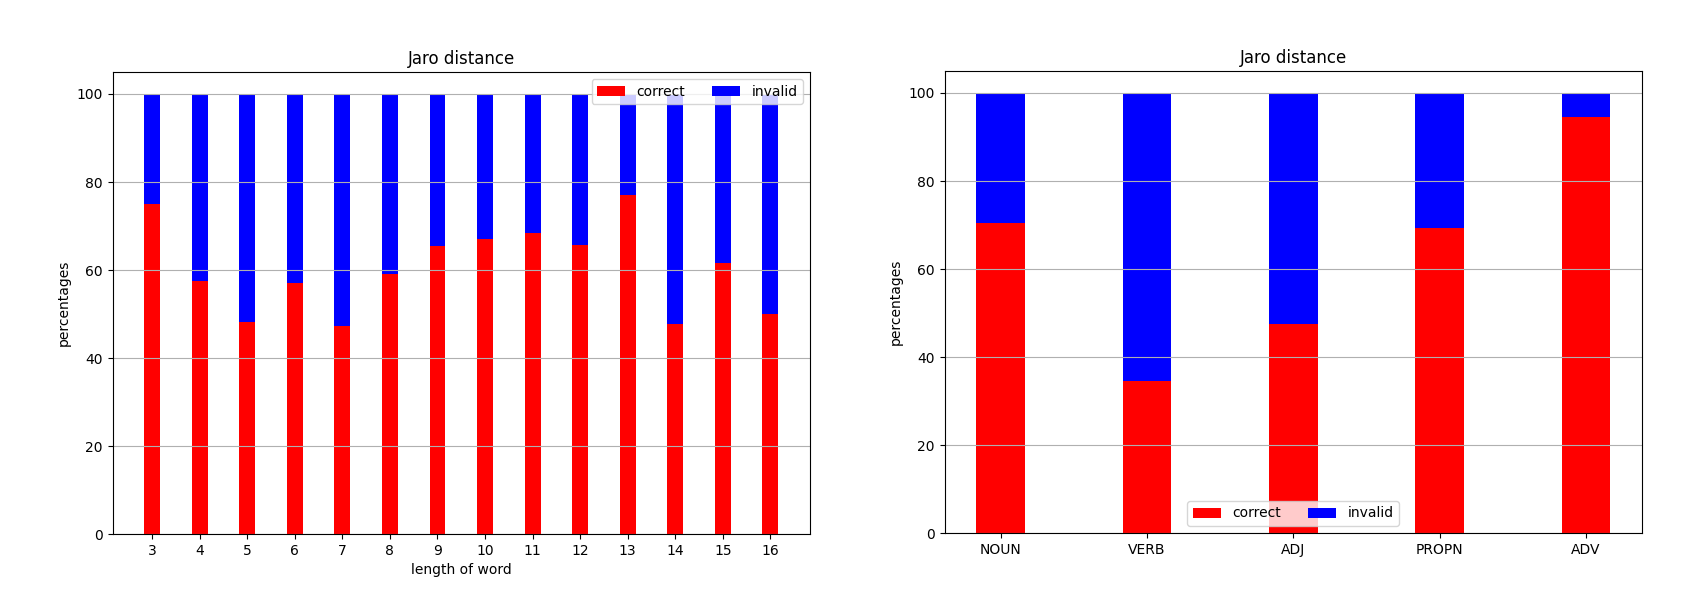
\includegraphics[width=1\textwidth]{Jaro_res.png} \\ Результаты тестирования расстояния Джаро ($J$)}
\label{ris:Jaro.png}
\end{figure}

\begin{figure}[htbp]
\center{\includegraphics[width=1\textwidth]{Jaro–Winkler_res.png} \\ Результаты тестирования расстояния Джаро-Винклера ($JW(2, 0.4, 0.7)$)}
\label{ris:Jaro-Winkler.png}
\end{figure}

\newpage

\begin{figure}[htp]
\center{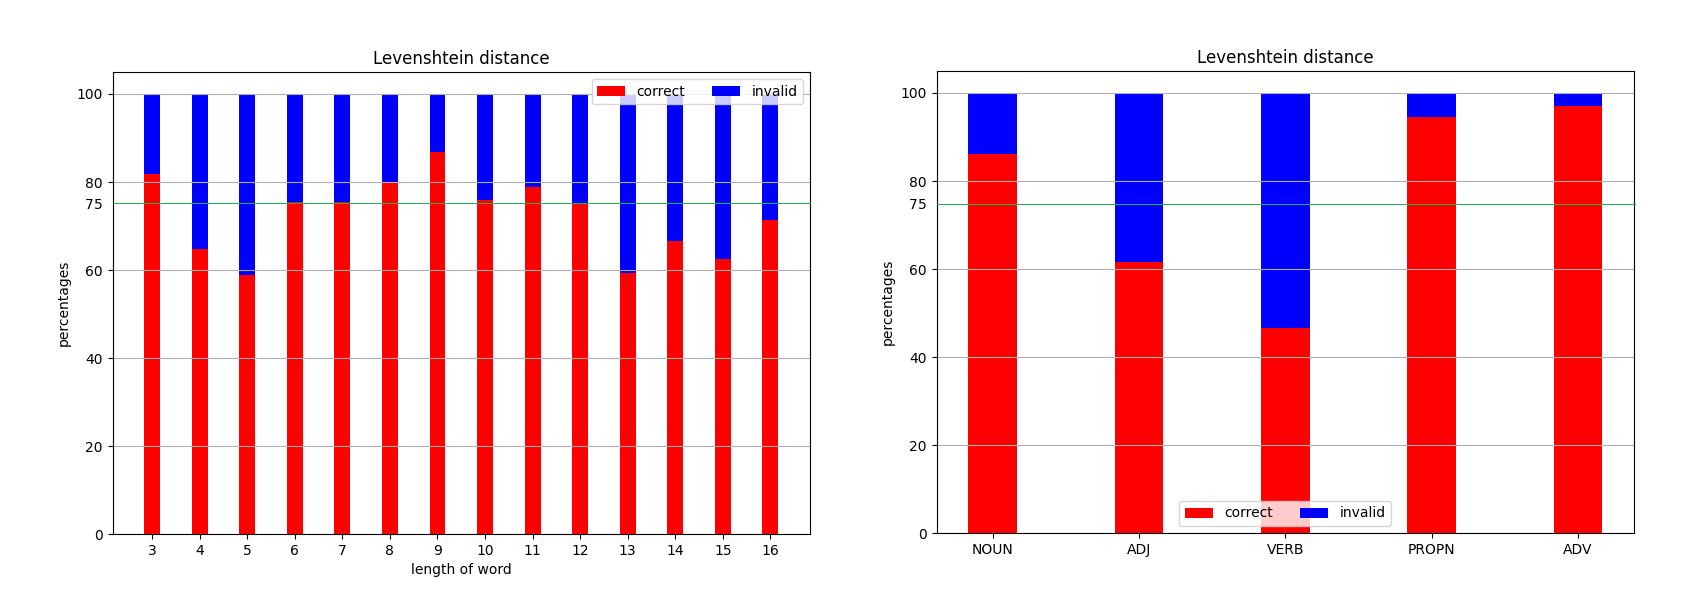
\includegraphics[width=1\textwidth]{Levenshtein_res.png} \\ Результаты тестирования расстояния Левенштейна ($L$)}
\label{ris:Levenshtein.png}
\end{figure}

Из приведенных выше данных можно увидеть схожую структуру распределения верных ответов. Заметно, что точность для слов длины 3 у всех метрик примерно на одном уровне и выше среднего значения, это может быть связано с тем, что слова такой длины являются довольно уникальными в том, что нормальные формы различных слов, скорее всего, содержать совершенно разные символы из-за малости длины, что делает их легко отличимыми для всех метрик. 

Далее, на словах длины 4-7, виден спад точности на всех графиках ниже или на уровне средней точности, этот спад связан с недостатком всех метрик, который упоминался ранее, а именно то, что схожие слова малой длины получают лучшее значение метрики, чем схожие длинные слова, особенно данная проблема видна при использовании расстояния Джаро, где ,вплоть до слов длины 8, значение точности метрики не увеличивается.

Далее, на словах длины 8-12, виден подъем значения точности, так как, начиная со слов  средней длины, недостатки метрик, из-за которых проседала точность коротких слов, уже не оказывают столь сильного влияния, поэтому на данном промежутке длины слов все метрики показывают результат выше или на уровне средней точности.

И наконец, на словах длины 13-16, есть некоторые различиня в поведении метрик, например, при использовании расстояния Левенштейна точность оценки снижается сильно ниже среднего, это может быть связано с тем, что количество минимальных операций приведения формы слова к нормальной форме, на основе которого и измеряется расстояние Левенштейна, увеличивается по мере роста длины слова, из-за чего увеличивается вероятность спутать иную нормальную форму с нужной. При использовании расстояния Джаро или расстояния Джаро-Винклера значение точности уровне среднего, кроме слов длины 14, что, скорее всего, является статистической погрешностью.

\newpage

При рассмотрении графиков распределения верных ответов от части речи видна очень схожая структура. Значение верных ответов сильно ниже при лемматизации глаголов и прилагательных, это может быть связано с тем, что у этих частей речи наиболее разнообразны формы слова, что и влияет на качество ответов.

\section{Представление словарей в памяти}
\quad Одной из проблем алгоритмов леммализации является представление словарей в памяти компьютера. Понятно, что эффективное представление должно занимать не слишком много места, а главное чтобы для них существовали алгоритмы позволяющие уменьшать количество потенциальных нормальных форм, используя информацию из полученной формы слова. Рассмотрим несколько таких видов структур.

\subsection{Префиксное дерево}
\quad Префиксное дерево представляет собой структуру, с топологической точки зрения являющуюся направленным деревом. Данное дерево имеет единственный корень. Каждый узел дерева может иметь неогранниченое количество потомков. Каждый узел хранит список уникальных для узла ключей и потомков, соответствующих каждому ключу, а также флаг. Иногда узел хранит также дополнительное значение.

При заполнении дерева каждому слову соответсвует путь начинающийся из корня и заканчивающийся в узле с истинным флагом, ключи между узлами в данной цепочке выступают символы слова. Если слова имеют одинаковый префикс, то порожденная ими цепочка будет иметь совпадающие узлы, за счет которых и экономится память.

\begin{figure}[htp]
\center{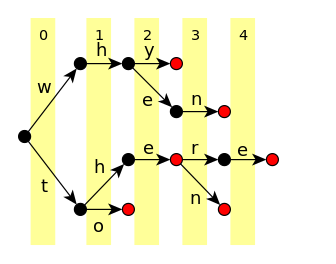
\includegraphics[width=0.6\textwidth]{Prefix_Trie.png} \\ Пример префиксного дерева. Красным помечены узлы с истинным флагом}
\label{ris:Prefix_Trie.png}
\end{figure}

Очевидно, что по памяти данная структура не превосходит простое хранение всех элементов словаря, а при большом количестве слов может значительно сократить затраты. Также один из плюсов префиксного дерева это быстрая проверка существования слова в словаре за $O(n)$, где $n$ - длина слова.

\subsection{Детерминированный ациклический конечный автомат}
\quad Детерминированный конечный автомат(DFA) - набор из 5 элементов: $M = (Q, \Sigma, \delta, q_0, F)$, где $Q$ - конечное множество состояний, $\Sigma$ - конечное множество возможных входных символов (алфавит), $\delta: Q \times \Sigma \longrightarrow Q$ - функция перехода, $q_0 \in Q$ - начальное состояние, $F \subset Q$ - множество допускающих состояний.

Изначально автомат находится в стартовом состоянии $q_0$. Автомат считывает входные символы  
$r_1, r_2, \dots, r_n \in \Sigma$, переходя в состояние $q_1, q_2, \dots, q_n \in Q$, где $q_i = \delta(q_{i-1}, r_i)$, \\ $\; \forall \: i = \overline{1, n}$. Процесс продолжается до тех пор, пока не будет достигнут конец входного слова.

Будем говорить, что автомат $M$ допускает слово $r_1 r_2\dots r_n$, если для каждого символа определена $\delta(q_{i-1}, r_i)$ и $q_n \in F$. Множество всех слов, которые допускает автомат $M$ будем называть языком автомата $L(M)$.

Теперь не сложно заметить, что префиксное дерево является детерминированным ациклическим конечным автоматом(DAFSA), где $Q$ - множество узлов, $\Sigma$ - символы алфавита, $\delta$ - ребра дерева, $q_0$ - корневой узел, $F$ - узлы с истинным флагом, а так как префиксное дерево топологически является деревом, то оно не имеет циклов. Если к DAFSA применить алгоритм минимизации конечных автоматов, который уменьшает количество возможных состояний $Q$ и при этом множество $L(M)$ оставляет неизменным, можно добиться еще большей экономии памяти.


\begin{figure}[htp]
\center{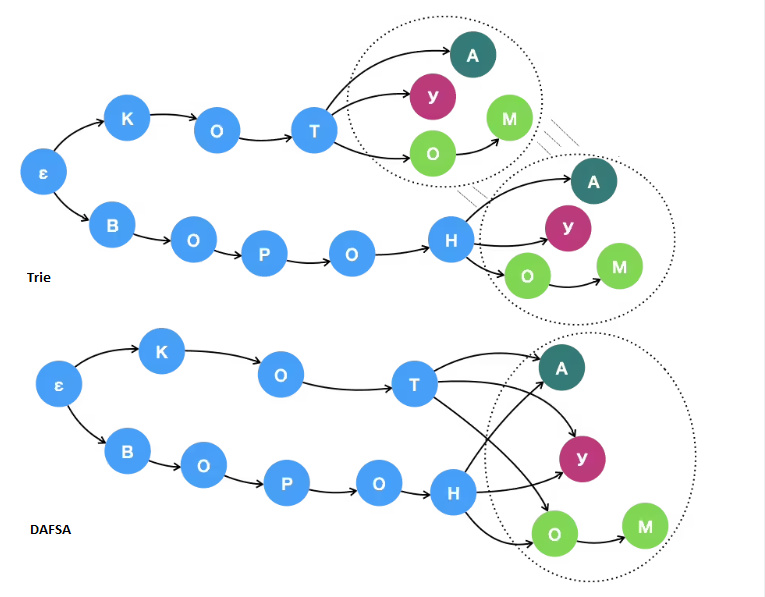
\includegraphics[width=0.56\textwidth]{MinDAFSA.png} \\ Пример минимизации префиксного дерева}
\label{ris:MinDAFSA.png}
\end{figure}

Стоит отметить, что проверка допустимости слова, то есть проверка существования слова в словаре, также, как и в префиксных деревьях выполняется за $O(n)$, но при этом теперь невозможно хранить дополнительную информацию в узлах, из-за чего всю вспомогательную информацию нужно хранить в отдельнух структурах.

\subsection{Пример использования префиксного дерева в алгоритме лемматизации}





\newpage

\section{Современные алгоритмы лемматизации}

\section{Ссылки}

\hypertarget{r1} $[1]$ \href{https://github.com/Dx-by-Dy/Python-programs/tree/main/NLP/Datasets}{\textcolor{blue}{Используемые датасеты для практического тестирования алгоритмов}}

\end{document}